\documentclass{article}
\usepackage[utf8]{inputenc}
\usepackage{parskip}
\usepackage{graphicx}
\usepackage{subcaption}

\title{ANNDA - Lab 2}
\author{Niels Agerskov, Lukas Bjarre, Gabriel Carrizo}
\date{December 2017}

\begin{document}

\maketitle
\pagebreak

\section{Batch Mode Training}

In this part of the lab we trained an RBF network to approximate two functions:

\begin{equation}
  f_1(x) = sin(2x)
\end{equation}
\begin{equation}
  f_2(x) = square(2x)
\end{equation}

Where $x \epsilon [0, 2\pi]$ which is sampled with a step sizeof 0.1. The function is consequently tested with $x_{test} = x+0.05$.

\begin{figure}[ht!]
    \centering
    \begin{subfigure}[t]{0.4\textwidth}
        \centering
        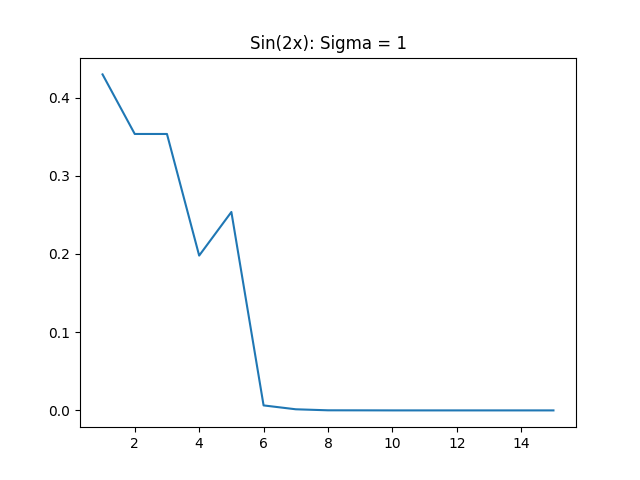
\includegraphics[width=1\textwidth]{plots/batch/batch_error_sin2x.png}
        \caption{}
    \end{subfigure}
    \begin{subfigure}[t]{0.4\textwidth}
        \centering
        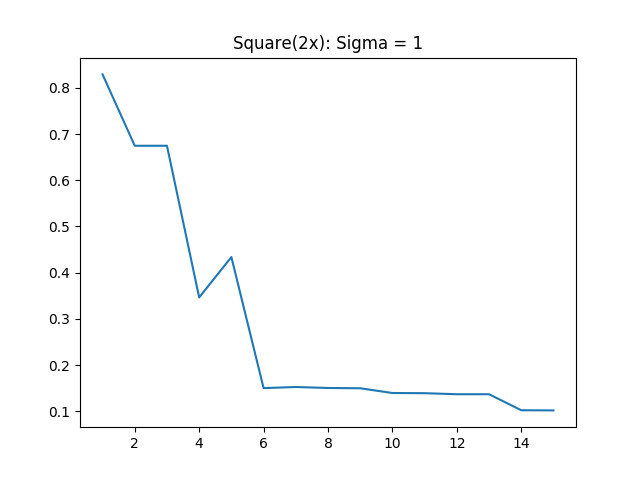
\includegraphics[width=1\textwidth]{plots/batch/batch_error_square2x.png}
        \caption{}
    \end{subfigure}
    \begin{subfigure}[t]{0.4\textwidth}
        \centering
        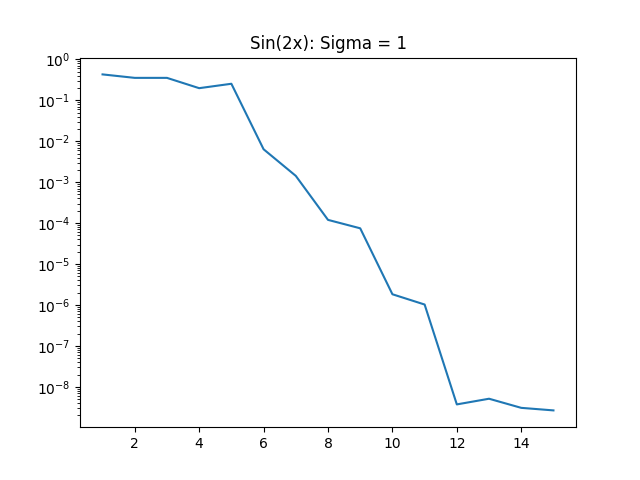
\includegraphics[width=1\textwidth]{plots/batch/batch_error_sin2x_log.png}
        \caption{}
    \end{subfigure}
        \begin{subfigure}[t]{0.4\textwidth}
        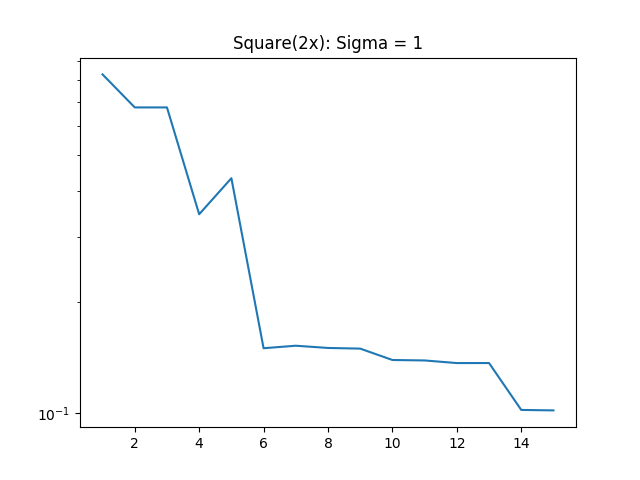
\includegraphics[width=1\textwidth]{plots/batch/batch_error_square2x_log.png}
        \caption{}
    \end{subfigure}
    \begin{subfigure}[t]{0.4\textwidth}
        \centering
        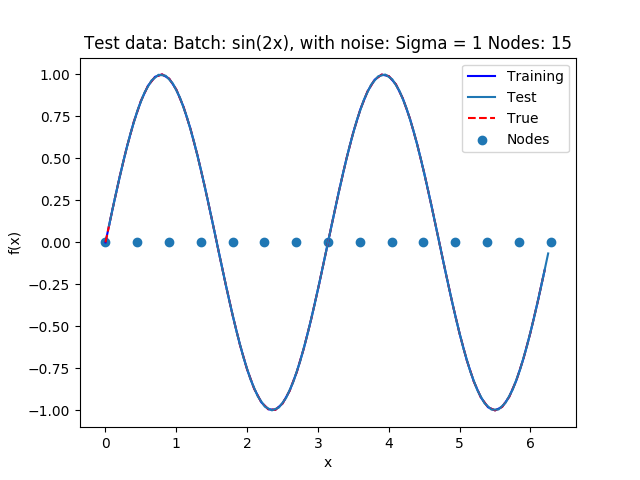
\includegraphics[width=1\textwidth]{plots/batch/best_sin2x.png}
        \caption{}
    \end{subfigure}
        \begin{subfigure}[t]{0.4\textwidth}
        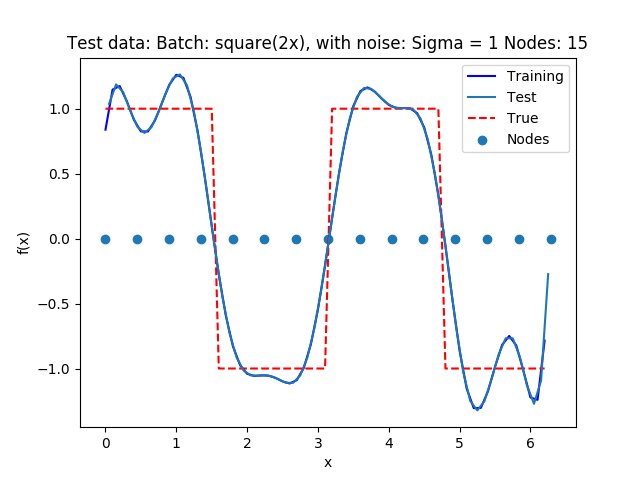
\includegraphics[width=1\textwidth]{plots/batch/best_square2x.png}
        \caption{}
    \end{subfigure}
\end{figure}

\begin{figure}[ht!]
    \centering
    \begin{subfigure}[t]{0.4\textwidth}
        \centering
        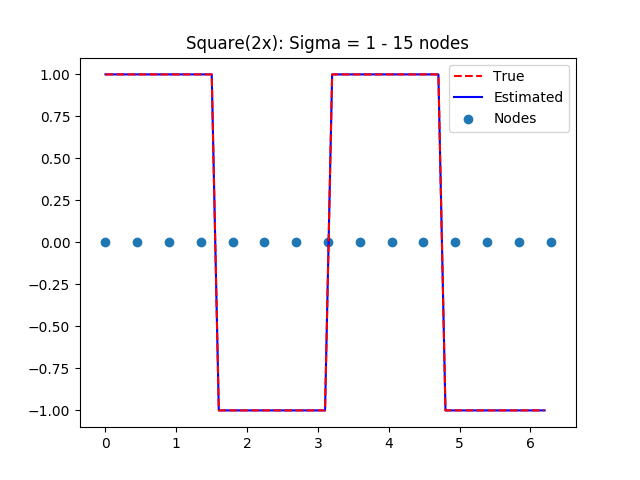
\includegraphics[width=1\textwidth]{plots/batch/best_square_cheat.png}
        \caption{}
    \end{subfigure}
    \begin{subfigure}[t]{0.4\textwidth}
        \centering
        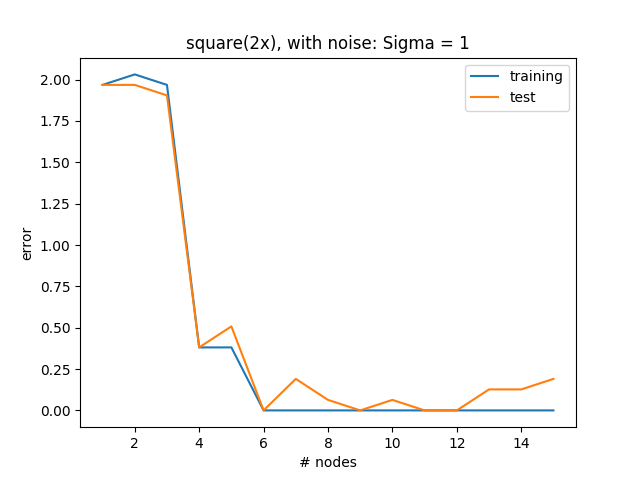
\includegraphics[width=1\textwidth]{plots/batch/square_error_sign}
        \caption{}
    \end{subfigure}
\end{figure}


\end{document}
